\section{Dynamisk programmering}
Dynamisk programmering og grådighet  er to \textit{designmetoder} – generelle ideer som man kan bygge opp algoritmer rundt. De brukes som regel når vi har et optimaliseringsproblem, altså et problem hvor det finnes flere løsninger som i og for seg er gyldige, men vi ønsker å finne den beste av dem. To viktige begreper i dette kapittelet er optimal struktur og overlappende delproblemer.
\\\\
\textbf{Optimal substruktur} er den optimale løsningen på problemet, og består av optimale løsninger på underproblemer. Det vil si at du kan bruke løsninger på delproblemer for å finne løsningen på hele problemet.

\begin{boxed}
Å finne det n'te Fibonacci-tallet er et eksempel på et problem med optimal substruktur. Hvis vi vet $f(n - 1)$ og $f(n - 2)$ kan vi bruke dette til å finne $f(n)$.
\end{boxed}

\noindent Et annet eksempel er korteste-vei-problemer. Den korteste veien fra A via B til C består av den korteste veien fra A til B og den korteste veien fra B til C. 
\\\\
\textbf{Overlappende delproblemer} bør man se opp for. En naiv splitt og hersk-algoritme brukt på et slikt problem vil løse samme delproblem mange ganger. Dynamisk programmering angriper problemet ved å løse de enkleste delproblemene først, og deretter kombinere løsningene på disse for å løse de større delproblemene, og til slutt hele problemet.

\begin{boxed}
For å finne $f(n)$ må vi først finne $f(n - 1)$ og $f(n - 2)$. En naiv rekursiv metode vil regne ut disse hver for seg:\\
\newline
$f(n - 1)$ = $f(n - 2)$ + $f(n - 3)$\\ 
$f(n - 2)$ = $f(n - 3)$ + $f(n - 4)$\\ 
\newline
Allerede her kommer det fram to overlappende delproblemer, $f(n - 2)$ og $f(n - 3)$. Disse vil her regnes ut flere ganger, og utregningen innebærer enda flere rekursive kall. 
\end{boxed}

Hvis du kommer over et problem med optimal substruktur og overlappende delproblemer, er det stor mulighet for at dette er en oppskrift du kan følge for en effektiv algoritme:
\begin{enumerate}
    \item Bli sikker på at problemet har optimal substruktur og overlappende delproblemer.
    \item Løs problemet for eller de mest trivielle situasjonen(e). Bruk så disse til å finne de nest vanskeligste osv.
    \item Hvilke valg har du? Hva bør du velge i de forskjellige tenkelige situasjonene?
    \item sett opp et skjema og fyll inn for noen tall.
    \item Programmer.
\end{enumerate}

\begin{boxed}
Per er veldig dårlig i rettskrivning. Han vet ikke om han skal skrive "gullerot" eller "gulrot". Per er ikke alene, blant annet har de som designer søkemotorer på internett oppdaget at det er mange som han. I stedet for at han får null treff på "gullerot" er det et ønske om at han skal få opp et spørsmål om han ikke heller vl søke på "gulrot" eller andre lignende ord. Denne funksjonen er også nyttig for de som skriver touch litt fortere enn de klarer.
\\\\
Søkemotoren trenger da blant annet et program som sammenligner ord. Det er dette vil skal lage. Som eksempel bruker vi "gullerot" og "gulrot". Vi ønsker å finne ut hvor stor forskjell det er på disse to skrivemåtene, dvs. hvor mange editeringer vi må gjøre for å få "gullerot" til å bli "gulrot". 

\begin{enumerate}
    \item \textbf{Har problemet optimal substruktur?} Ja. F.eks. er et delproblem å finne ut hvor mange editeringer du trenger for å forandre \textit{gulro} til \textit{gulle}. Hvis vi vet svaret på dette, er oppgaven litt enklere, altså optimal substruktur.\newline
    \textbf{Har problemet overlappende delproblemer?} La oss si at vi har funnet ut hvor mange editeringer som skal til for å forandre \textit{gulle} til \textit{gulro}. Dette vil vi bruke både når vi skal finne ut hvor mange editeringer som skal til for å forandre \textit{gul} til \textit{gulrot}, \textit{gull} til \textit{gullro} og \textit{gull} til \textit{gullrot}. Dvs. dette problemet, som vi nå har løsningen på er et underproblem til alle disse tre. (Men ingen av disse tre er delproblemer av hverandre.) Altså har vi overlappende delproblemer.
    
    \item De mest trivielle delproblemene er antall editeringer for å forandre \textit{g} til \textit{g}, \textit{gu} ... og \textit{gulerot} og andre veien; \textit{g}, \textit{gu}, \textit{gul}, \textit{gull} ... og \textit{gullerot} til \textit{g}.\newline
    \newline
    Dette kan settes inn i en matrise. Vi kaller matrisen \textit{c}. Verdien i f.eks. rute $c(2,3)$ er minste antall editeringer som skal til for å forandre \textit{gul} til \textit{gulr}.
    
    \item Spørsmålet er hvordan vi finner ut verdien i \textit{c(i,j)}. La oss si at vi har regnet ut de tre nærmeste delproblemene A, B og C. Vi har da tre muligheter for verdien $c(i,j)$:
    \begin{enumerate}
        \item \textbf{bokstav i = bokstav j:} Siste bokstav i ordene vi ser på er like, så vi trenger ikke gjøre noen nye editeringer; vi kan bare se på resten av ordene. For eksempel, hvis ordene er "gullerot" og "gulrot", kan vi se bort fra \textit{t}'en, fordi hvis vi finner ut hvor mange editeringer det kreves for å gjøre om "gullero" til "gulro", vet vi at det vil ta like mange for å omforme "gullerot" til "gulrot". Altså blir det $c(i,j) = c(i - 1, j - 1) = A$.
        \item \textbf{bokstav i $\neq$ bokstav j:} Her er det to muligheter:
        \begin{enumerate}
            \item Vi kan ta verdien i B of legge til 1. Dette tilsvarer å erstatte bokstav \textit{i} med bokstav \textit{j}.
            \item Vi kan ta verdien i \textit{c} og legge til 1. Dette tilsvarer å slette bokstav \textit{i}.
        \end{enumerate}
        Vi velger selvsagt det som gir alternativet som tilsvarer færrest editeringer.
        \item Det er bare å fylle inn tabellen.
        \begin{figure}[H]
        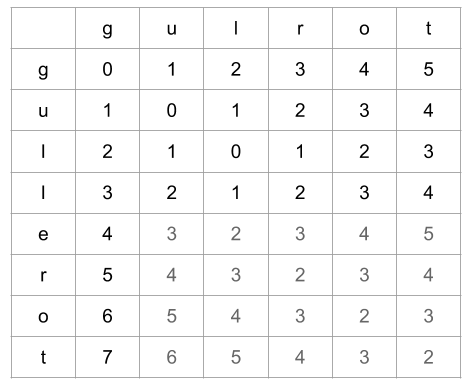
\includegraphics[scale=0.45]{images/dp}
        \centering %centering the image
        \caption{Dynamisk programmering}
        \label{fig:dp}
        \end{figure}
        
    \end{enumerate}
\end{enumerate}

\end{boxed}

\subsection{Lengste felles understreng}
\subsection{Rod-cutting}